% !TEX root = ../main.tex
%-------------------------------------------------------------------------------
%-------------------------------------------------------------------------------
\begin{frame}\begin{center}
		\LARGE\textbf{High-performance libraries}
\end{center}\end{frame}
%-------------------------------------------------------------------------------
%-------------------------------------------------------------------------------
\begin{frame}\textbf{Vectorization}\vspace{0.3cm}

\begin{itemize}\setlength\itemsep{1em}
    \item Vectorization is when a CPU is provided with multiple pieces of data at a time and is able to operate on all of them at once. This sort of CPU instruction is known as SIMD (Single Instruction, Multiple Data).
\end{itemize}

\end{frame}
%-------------------------------------------------------------------------------
%-------------------------------------------------------------------------------
\begin{frame}\textbf{Practical illustration}\vspace{0.3cm}
  	\begin{figure}[htp]\centering
      \scalebox{0.2}{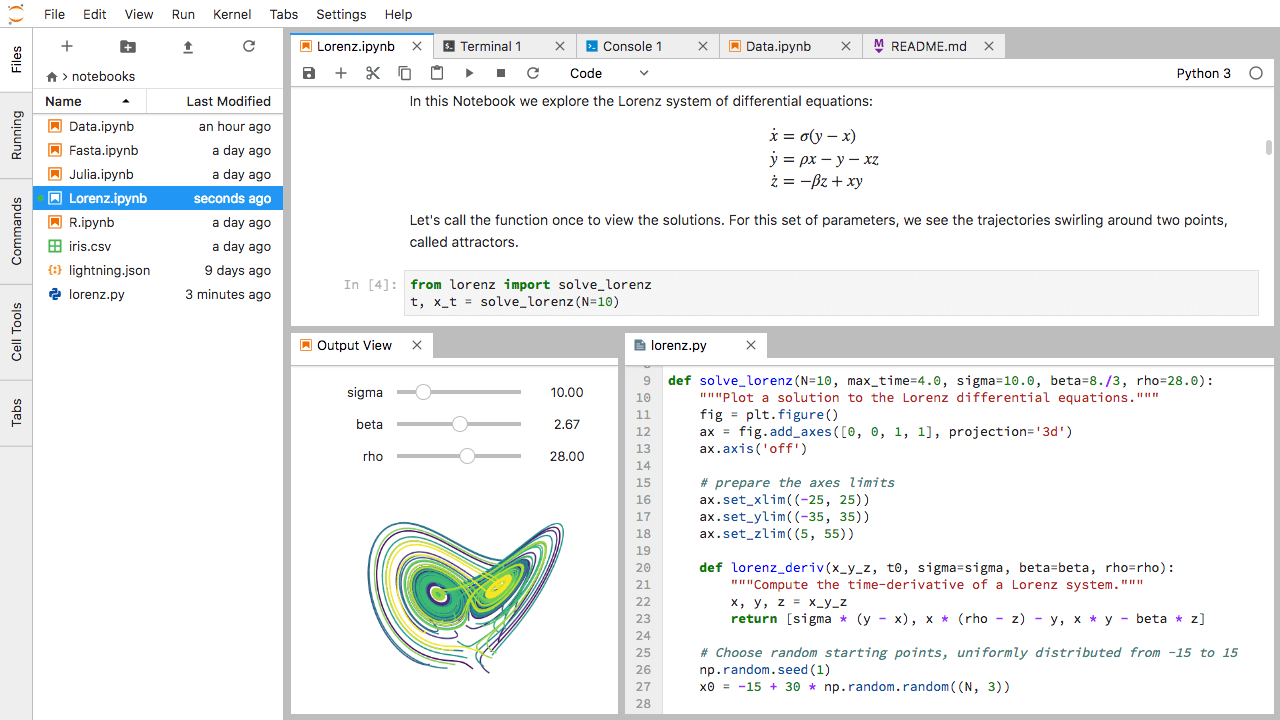
\includegraphics{fig-jupyterlab}}
  	\end{figure}
\end{frame}
%-------------------------------------------------------------------------------
%-------------------------------------------------------------------------------
